\documentclass[10pt, colorlinks=true, urlcolor=blue]{beamer}

% Themes and colors for a professional look
\usetheme{Madrid}
\usecolortheme{seagull}
\setbeamercolor{title}{fg=white,bg=blue!80!black}
\setbeamercolor{frametitle}{fg=white,bg=blue!70!black}
\setbeamercolor{block title}{fg=white,bg=blue!80!black}
\setbeamercolor{block body}{bg=blue!5!white}
\setbeamerfont{title}{size=\fontsize{12}{16}\selectfont}

% Customize the footline layout
\setbeamertemplate{footline}
{
  \leavevmode%
  \hbox{%
    % Left field (author or custom text)
    \begin{beamercolorbox}[wd=0.25\paperwidth,ht=2.5ex,dp=1ex,center]{author in head/foot}%
      \usebeamerfont{author in head/foot}\insertshortauthor
    \end{beamercolorbox}%
    % Middle field (title)
    \begin{beamercolorbox}[wd=0.5\paperwidth,ht=2.5ex,dp=1ex,center]{title in head/foot}%
      \usebeamerfont{title in head/foot}\insertshorttitle
    \end{beamercolorbox}%
    % Right field (page number)
    \begin{beamercolorbox}[wd=0.25\paperwidth,ht=2.5ex,dp=1ex,center]{date in head/foot}%
      \usebeamerfont{date in head/foot}\insertframenumber/\inserttotalframenumber
    \end{beamercolorbox}%
  }%
}

% Set hyperlink colors
\hypersetup{
    colorlinks=true,    % Enable colored links
    urlcolor=blue,      % Color for URLs
    linkcolor=blue      % Color for internal links (optional)
}

\usepackage{minted}

\title{Python Mutability Visually Explained Using `memory\_graph'}
\author{Bas Terwijn}
\titlegraphic{
\vspace{-3.5em} % Adjust this value as needed
  \makebox[\textwidth]{%
  \begin{tabular}{c c}
    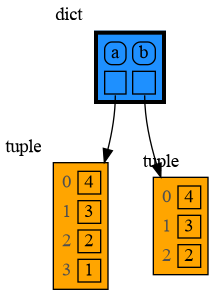
\includegraphics[height=0.35\textwidth]{figures/immutable.png} &
    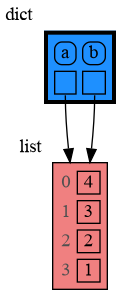
\includegraphics[height=0.35\textwidth]{figures/mutable.png} \\
      &  \\
    \multicolumn{2}{c}{
      
\includegraphics[width=0.6\textwidth]{figures/uva.png}
    }
  \end{tabular}
}
}
\date{}

\begin{document}

\begin{frame}
    \titlepage
\end{frame}

%% \begin{frame}{Content}
%%   We will cover these \href{https://docs.python.org/3/reference/datamodel.html}{\texttt{Python Data Model}} topics:
%%   \begin{itemize}
%%   \item Mutability of Types
%%   \item References to Values
%%   \item Coping Values
%%   \end{itemize}

%%   \vspace{2em}
  
%%   These concepts are fundamental to Python programming.
%%   \begin{itemize}
%%     \item without a solid understanding you cannot avoid certain bugs
%%   \end{itemize}

%%   \vspace{2em}
  
%%   We will use visualization tools to help build a solid understanding:
%%   \begin{itemize}
%%   \item \href{https://pypi.org/project/memory-graph/}{\texttt{memory\_graph}}
%%   \item \href{https://pythontutor.com/}{\texttt{Python Tutor}}
%%   \end{itemize}

%%   \vspace{2em}

%%   We finish with an exercise with which you can test your understanding.
%% \end{frame}


\begin{frame}{Immutable and Mutable Types}
  \begin{block}{Python Types}
    Python has two distinct categories of types: Immutable, Mutable
  \end{block}
  
  \vspace{2.4em}
  
  \textbf{Immutable} Types: \texttt{bool}, \texttt{int}, \texttt{float}, \texttt{complex}, \texttt{str}, \texttt{tuple}, \texttt{bytes}, \texttt{frozenset} \\
  
  \vspace{-0.8em}
  A value of an immutable type \textbf{cannot} be mutated in place. \\
  So when it is changed, \textbf{an} automatic copy is made. \\
  
  \vspace{2.0em}
  
  \textbf{Mutable} Types: \texttt{list}, \texttt{set}, \texttt{dict}, \texttt{classes}, \dots (most other types) \\
  
  \vspace{-0.8em}
  A value of a mutable type \textbf{can} be mutated in place. \\
  So when it is changed, \textbf{no} copy is made.
\end{frame}

\begin{frame}{Rational behind Mutable and Immutable types}
 
  \textbf{Mutable} Types: \texttt{list}, \texttt{set}, \texttt{dict}, \texttt{classes}, \dots (most other types)
  \begin{itemize}
  \item values need to change often
  \item and values can be large
  \end{itemize}
  Therefore, it is inefficient to copy a value each time we change it.
  
  \vspace{3em}
  
  \textbf{Immutable} Types: \texttt{bool}, \texttt{int}, \texttt{float}, \texttt{complex}, \texttt{str}, \texttt{tuple}, \texttt{bytes}, \texttt{frozenset}
  \begin{itemize}
  \item values generally don't need to change as much
  \item or values are small
  \end{itemize}
  Therefore, an automatic copy is less of a concern.

  \vspace{2em}
  
\end{frame}

\begin{frame}[fragile]
  \frametitle {Sharing Mutable Values}
  When two variables share a value of \textbf{mutable} type, changing one changes the other.
  \vspace{1em}
\begin{columns}
  \column{0.3\textwidth}
  \begin{minted}[fontsize=\small]{python}
           a = [4, 3, 2]
           b = a
           a += [1]
    \end{minted}
  \column{0.7\textwidth}
  \begin{center}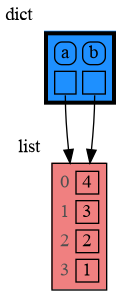
\includegraphics[width=0.25\textwidth]{figures/sharing.png}\end{center}
\end{columns}
\vspace{1em}
Sometimes we want this but other times we don't. Then we have to \textbf{make a copy} so that each variable has its own independent value.
\end{frame}


\begin{frame}[fragile]
  \frametitle{Copying Values}
  When ``copying'' a value of \textbf{mutable} type, consider the amount of sharing needed:
  \vspace{-1em}
\begin{columns}
  \column{0.4\textwidth}
  \begin{minted}[fontsize=\small]{python}
      a = [ [1, 2], ['x', 'y'] ]
      c1 = a
      c2 = copy.copy(a)
      c3 = copy.deepcopy(a)
    \end{minted}
  \column{0.6\textwidth}
    \begin{center}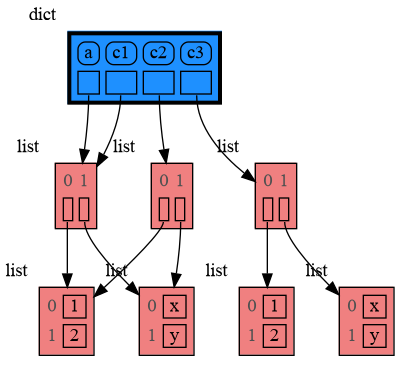
\includegraphics[width=0.7\textwidth]{figures/copy.png}\end{center}
\end{columns}
    \begin{itemize}
        \item \textbf{c1: Assignment,} nothing is copied, all the values are shared
        \item \textbf{c2: Shallow Copy,} only the value referenced by the first reference is copied, all the underlying values are shared
        \item \textbf{c3: Deep Copy,} all the values are copied, nothing is shared
        \item \ \ \, \,\, \textbf{Custom Copy,} alternatively write your own custom copy logic
    \end{itemize}
\end{frame}

\begin{frame}[fragile]
\frametitle{Function Calls}
  A function called with a \textbf{mutable} value can change that value.
  \begin{itemize}
  \item If you don't want that, make a copy.
  \end{itemize}

  \begin{columns}
    \column{0.4\textwidth}
    \begin{minted}[fontsize=\small]{python}
      def add_one(a, b, c):
         a += [1]
         b += (1,)
         c += [1]
         
      a = [4, 3, 2]
      b = (4, 3, 2)
      c = [4, 3, 2]
      add_one(a, b, c.copy())
    \end{minted}
    \column{0.6\textwidth}
    \begin{center}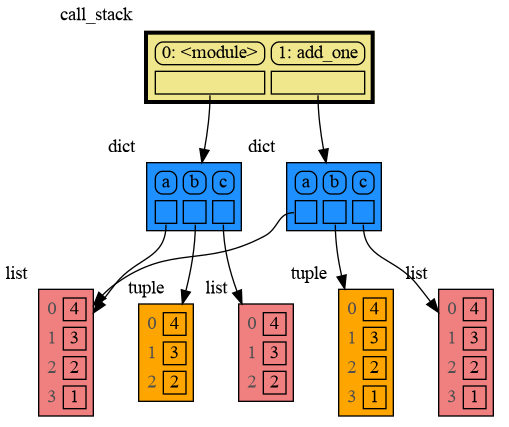
\includegraphics[width=0.9\textwidth]{figures/function_call.png}\end{center}
  \end{columns}
\end{frame}

\begin{frame}{memory\_graph Debugger Setup}
  \vspace{-1em}
  Debugger Setup:
  \begin{itemize}
  \item install \href{https://pypi.org/project/memory-graph/}{\texttt{memory\_graph}} and \href{https://graphviz.org/download/}{\texttt{Graphviz}}
  \item open Python source file in Visual Studio Code
  \item add line: \\ \ \ \ {\footnotesize \mintinline{python}{import memory_graph as mg}}
  \item set a breakpoint and start the \href{https://code.visualstudio.com/docs/python/debugging}{\texttt{vscode debugger}}
  \item add watch: \\ \ \ \ {\footnotesize \mintinline{python}{mg.render(mg.stack_vscode(), 'debug.pdf')}}
  \item manually open file 'debug.pdf', resize window,  and set 'Always on Top'
  \end{itemize}
  
  \vspace{1.8em}
  
  Adobe Acrobat Reader Problem: doesn't refresh and blocks updates to PDF file
  \begin{itemize}
  \item install a refreshing PDF reader as your 'Default PDF Reader': \\ \ \ \
    \href{https://www.sumatrapdfreader.org/}{\texttt{SumatraPDF}},
    \href{https://okular.kde.org/}{\texttt{Okular}}, ...
  \item or use a refreshing viewer for an image file: \\
\ \ \ {\footnotesize \mintinline{python}{mg.render(mg.stack_vscode(), 'debug.svg')}} \\
\ \ \ {\footnotesize \mintinline{python}{mg.render(mg.stack_vscode(), 'debug.png')}}
  \end{itemize}
\end{frame}

\begin{frame}[fragile]\frametitle{memory\_graph Non-Debugger Setup}
  Non-Debugger Setup:
  \begin{itemize}
  \item install \href{https://pypi.org/project/memory-graph/}{\texttt{memory\_graph}} and \href{https://graphviz.org/download/}{\texttt{Graphviz}}
  \item open Python source file in any editor
  \item add line: \\ \ \ \ {\footnotesize \mintinline{python}{import memory_graph as mg}}
  \item add this line to source code where you want to graph: \\
    \ \ \ {\footnotesize \mintinline{python}{mg.show(mg.stack())}}\\
    \ \ \ {\footnotesize \mintinline{python}{mg.render(mg.stack(), 'stack.pdf')}}\\
  \item or graph and block (Press \texttt{<Enter>} to continue...) using: \\
    \ \ \ {\footnotesize \mintinline{python}{mg.block(mg.show, mg.stack())}}\\
    \ \ \ {\footnotesize \mintinline{python}{mg.block(mg.render, mg.stack(), 'stack.pdf')}}\\
  \item see \href{https://pypi.org/project/memory-graph/}{\texttt{memory\_graph}} docs for examples and shorthand \href{https://github.com/bterwijn/memory_graph?tab=readme-ov-file#debugging-without-debugger-tool}{\texttt{alias functions}}
  \end{itemize}
\end{frame}


%% \begin{frame}{Python Tutor}
%%   Alternatively use: \href{https://pythontutor.com/}{\texttt{Python Tutor}}\\
%%   {\small Dr. Philip J. Guo, Associate Professor of Cognitive Science, University of California}
%%   \vspace{1em}\\
%%   Pros:
%%   \begin{itemize}
%%   \item no installation or setup required
%%   \item widely known
%%   \item supports: Python, Java, C, C++, JavaScript
%%   \item supports backwards debugging
%%   \item good graph stability over time
%%   \end{itemize}
%%   Cons: (\href{https://docs.google.com/document/d/13_Bc-l2FKMgwPx4dZb0sv7eMfYMHhRVgBRShha8kgbU/}{\texttt{Python Tutor Limitations}})
%%   \begin{itemize}
%%   \item only runs single file in a webbrowser
%%   \item limited program: size, runtime, memory use
%%   \item can only import standard library modules
%%   \item no reading/writing files or command-line arguments
%%   \end{itemize}
%% \end{frame}

\begin{frame}{Exercise 'band\_schedule.py'}
  \begin{itemize}
  \item Download: \href{https://raw.githubusercontent.com/bterwijn/memory_graph_videos/refs/heads/main/mutability/mutability.zip}{\texttt{mutability.zip}}
    \begin{itemize}
    \item slides.pdf
    \item src/
    \item exercise/
    \end{itemize}
  \item Mental Model: \begin{center}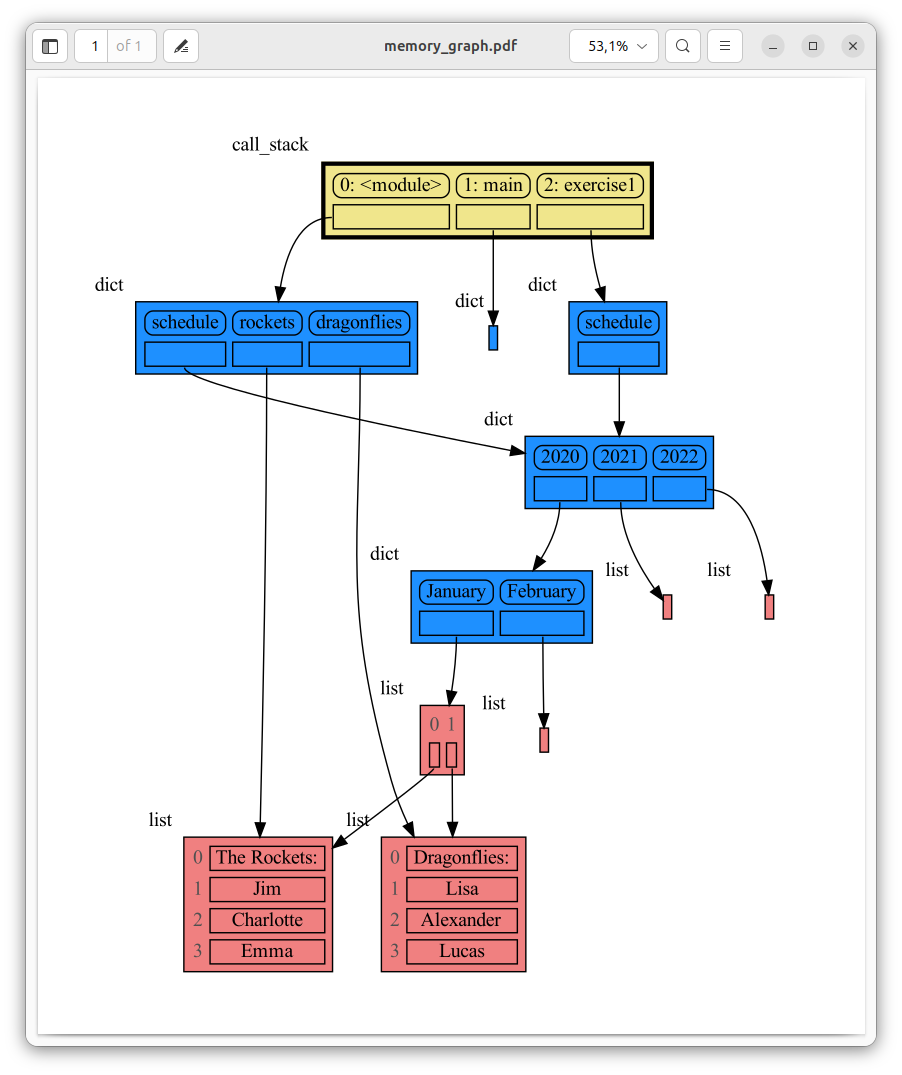
\includegraphics[width=0.4\textwidth]{figures/band_schedule.png}\end{center}
  \end{itemize}
\end{frame}

\end{document}
